\subsection{Общая информация об Apache Lucene и Solr}

The Apache Lucene -- это свободная библиотека для высокоскоростного полнотекстового поиска, написанная на Java. Может быть использована для поиска в интернете и других областях компьютерной лингвистики (аналитическая философия).

Основные возможности:

\begin{enumerate}
 \item Масштабируемая и высокоскоростная индексация
  \subitem свыше 95GB в час на современном оборудовании 
  \subitem требуется малый объем RAM — «heap» всего 1MB 
  \subitem размер индекса примерно 20-30 \% от размера исходного текста
 \item Мощный, точный и эффективный поисковый алгоритм
  \subitem ранжированный поиск — лучшие результаты показываются первыми
  \subitem множество мощных типов запросов: запрос фразы, wildcard запросы, поиск интервалов и т. д.
  \subitem поиск основанный на «полях» (таких как, заголовок, автор, текст)
  \subitem возможность сортировать по различным полям
  \subitem multiple-index поиск с возможностью объединения результатов
  \subitem возможность одновременного поиска и обновления индекса
 \item Кроссплатформное решение
  \subitem исходный код полностью написан на Java
  \subitem наличие портов на другие языки программирования
\end{enumerate}

Apache Solr – открытая корпоративная поисковая платформа, созданная на базе Apache Lucene. Основные возможности Apache Solr включают в себя мощный полнотекстовый поиск, подсветку результатов поиска, фасетный поиск, динамическую кластеризацию результатов, интеграцию с СУБД и поддержку индексирования документов разных форматов (например, MS Word и PDF). Также имеется возможность создания распределенной поисковой системы и репликация поискового индекса. 

Проект Apache Solr написан на Java  и запускается как самостоятельное приложение в контейнере сервлетов, например, на Apache Tomcat. Solr использует Lucene как поисковый механизм и имеет REST HTTP/XML и JSON интерфейс для взаимодействия с другими приложениями. 

\subsection{Установка Apache Solr}

Существует 3 готовых сборки Apache Solr из репозитория из них 2 для различных веб-серверов и 1 исходный код сервиса написанного на java. Cначала необходимо установить необходимый минимум програмных пакетов, которые позволят работать с Solr.

Как говорилось ранее поисковой сервис написан на языке java, поэтому в первую очередь необходимо установить JavaJDK, для этого открываем консоль и добавляем по очереди строки следующего содержания:

\begin{lstlisting}
apt-get update
apt-get install sun-java7-jdk
\end{lstlisting}

После установки JavaJDK скачиваем с официального сайта http://lucene.apache.org/solr/ исходники с поисковым сервисом актуальной версии, после чего разархивируем выполнив команду:

\begin{lstlisting}
tar -xzvf ./solr-4.10.2.tgz
\end{lstlisting}

Для запуска сервиса используетя скрипт написанный на java, чтобы его запустить необходимо перейти в папку example, которая находится \textasciitilde/solr-4.10.2/example/, и запустить скрипт. Пример как это проделать приведен ниже:

\begin{lstlisting}
cd ~/solr-4.10.2/example/
java -jar start.jar
\end{lstlisting}

Запустив сервис мы можем открыть его веб оболочку набрав в браузере http://localhost:8983/solr (рисунок \ref{ris:solr}).

\begin{figure}[h] 
\center{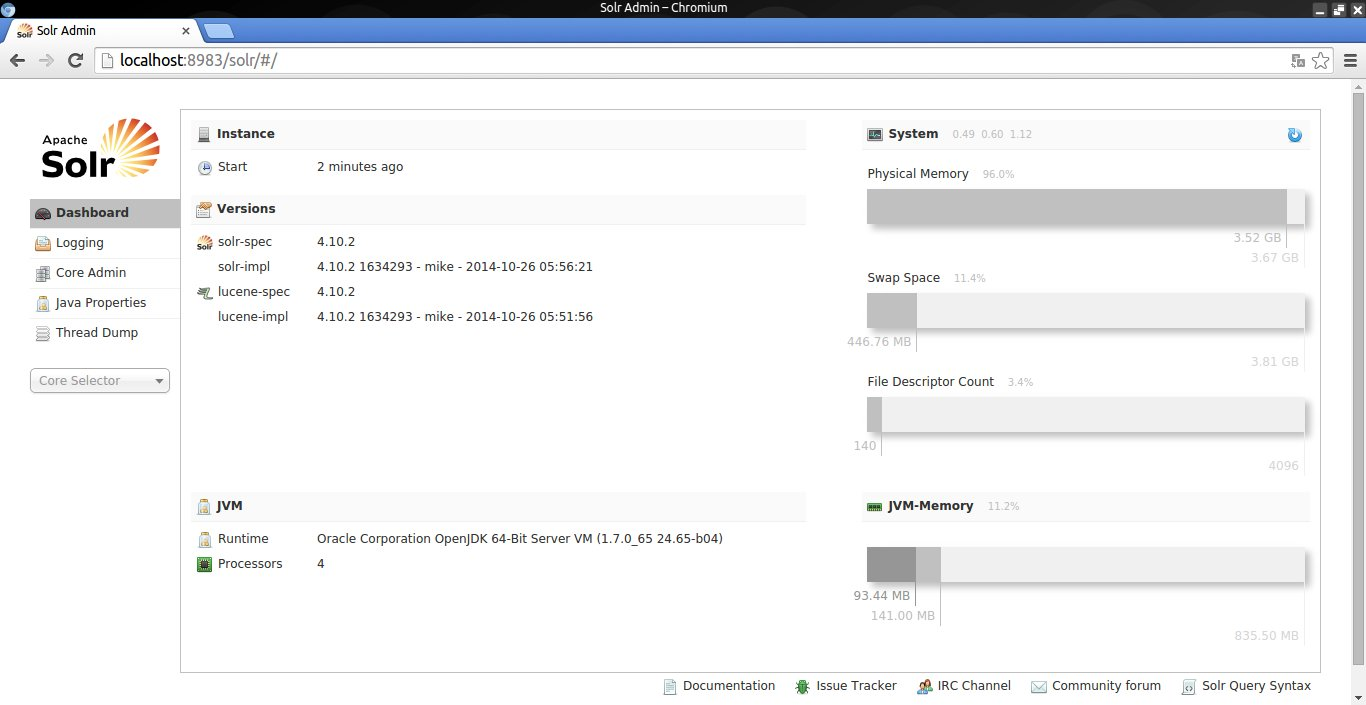
\includegraphics[width=1\linewidth]{solr}}
\caption{Веб-оболочка Solr}
\label{ris:solr}
\end{figure}
